\section{Tomasulo}

Tomasulo is a dynamic scheduling approach designed to enable continued execution despite dependencies.
Developed at IBM for the IBM 360/91, it emerged three years after the CDC 6600, aiming to achieve high performance without relying on specialized compilers.

\subsection{Tomasulo features}
In Tomasulo's design, control logic and operand buffers are decentralized, contrasting with the centralized approach of the Scoreboard algorithm. 
Buffers for operands are called Reservation Stations, where each instruction is represented as an entry.

Operands are replaced with values or pointers in a technique known as Register Renaming, which helps to avoid WAR and WAW hazards. 
Tomasulo's Reservation Stations provide more flexibility than traditional registers, enabling optimizations beyond compiler capabilities.
Results are distributed to other functional units via a Common Data Bus (CDB), which carries both data and its corresponding source. 
Additionally, load and store operations are treated as functional units within the algorithm.
\begin{figure}[H]
    \centering
    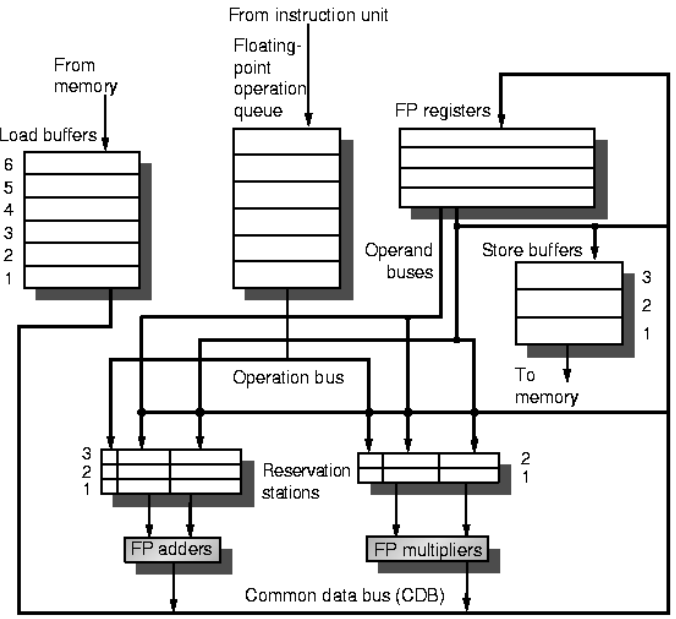
\includegraphics[width=0.75\linewidth]{images/tomasulo.png}
    \caption{Tomasulo data structure}
\end{figure}

\subsection{Tomasulo structure}
In Tomasulo, the following components are key:
\begin{itemize}
    \item \textit{Reservations Stations}: these stations include several components:
        \begin{itemize}
            \item \textit{Tag}: identifies the Reservation Station.
            \item \textit{OP}: specifies the operation to be executed.
            \item \textit{$V_j$, $V_k$}: values of the source operands.
            \item \textit{$Q_j$, $Q_k$}: pointers to Reservation Stations producing $V_j$, $V_k$.
            \item \textit{Zero value}: indicates that the source operand is already available in either $V_j$ or $V_k$.
            \item \textit{Busy}: indicates whether the Reservation Station is currently occupied.
        \end{itemize}
        Note that for each operand, only one of the $V$-field or $Q$-field is valid at a time.
    \item \textit{Register File and the store buffer}: both include a value and a pointer field. 
        The pointer field indicates the Reservation Station producing the result to be stored in the Register File or store buffer. 
        If the pointer is zero, it indicates no active instructions are producing the result, meaning the Register File or store buffer content is valid.
    \item \textit{Load buffers}: these buffers include an address field and a busy field. 
        They hold information related to memory address calculation for load and store operations. 
        Initially, they contain the instruction offset, and after address calculation, they store the effective address.
    \item \textit{Store buffers}: similar to load buffers, store buffers also feature an address field and manage store operations within the algorithm.
\end{itemize}

\subsection{Tomasulo control}
Tomasulo's algorithm unfolds across three main stages:
\begin{itemize}
    \item \textit{Issue}: retrieve an instruction from the instruction queue.
        If it's a floating-point operation, check for available Reservation Stations to avoid structural hazards.
        Perform Register Renaming to resolve WAW hazards, linking the Register File to instruction due to in-order issuance.
    \item \textit{Execution}: execute the instruction once both operands are available.
        If the operands are not ready, monitor the CDB for results, delaying execution until operands are ready to avoid RAW hazards.
        Multiple instructions may become ready simultaneously for the same FU.
        For load and store instructions, perform a two-step process: compute the effective address and store it in the load or store buffer. 
        Loads in the load buffer execute as soon as the MU is available, while stores in the store buffer wait until the value is ready before being sent to the MU.
    \item \textit{Write}: once the result is available, write it onto the CDB. 
        Distribute the result to the Register File and all Reservation Stations (including store buffers) waiting for this result. 
        Stores write data to memory during this stage, marking Reservation Stations as available for the next instructions.
\end{itemize}

\paragraph*{Load and store}
Loads and stores undergo effective address computation in a FU before proceeding to their respective load and store buffers. 
Loads require a second execution step to access memory before transitioning to the write result stage, sending the value from memory to the Register File and or Reservation Stations.
Stores complete their execution in the write result stage by writing data to memory. 

Load and store operations can be executed out of order, provided they access different memory locations. 
Hazards may occur if they access the same memory location.
To detect such hazards, the CPU must have computed the data memory addresses associated with any earlier memory operation. 
When a load executes out of order with a previous store, it's assumed the address was computed in program order.
nce the load address is computed, it's compared with the address fields in active store buffers. 
If there's a match, the load isn't sent to the Load buffer until the conflicting store completes.

Stores must check for matching addresses in both load and store buffers, a process called dynamic disambiguation, as opposed to the static disambiguation performed by the compiler. 
This approach requires significant hardware, including fast associative buffers in each Reservation Station, and a single CDB may limit performance.

\subsection{Summary}
\begin{table}[H]
    \centering
    \begin{tabular}{l|cc}
    \multicolumn{1}{c|}{\textbf{Feature}} & \textbf{Tomasulo}                   & \textbf{Scoreboard}  \\ \hline
    \textit{Issue window size}            & 14                                  & 5                    \\
    \textit{Structural hazards}           & No                                  & No                   \\
    \textit{WAW and WAR}                  & Implicit Register Renaming          & Stalls               \\
    \textit{Control type}                 & Distributed on Reservation Stations & Centralized          \\
    \textit{Results handling}             & Broadcasted from FUs                & Written to registers \\
    \textit{Loop unrolling}               & Yes                                 & No                  
    \end{tabular}
\end{table}
Both approaches distribute control and buffers with FUs, as opposed to centralizing them in the Scoreboard. 
In Tomasulo's method, Reservation Stations serve as buffers for pending operands. 
Registers in instructions are replaced by values or pointers to Reservation Stations through Register Renaming, avoiding WAR and WAW hazards. 
Tomasulo can use more Reservation Stations than registers, enabling optimizations beyond compiler capabilities.

Results are sent to FUs from Reservation Stations via a CDB that broadcasts results to all FUs. 
Additionally, load and store operations are treated as FUs with associated Reservation Stations. 
Tomasulo allows integer instructions to proceed past branches, enabling floating-point operations beyond the basic block in the floating-point queue.